
Race drivers follow a racing line for specific maneuvers. This line can be used as a reference path by the motion planner to assign time-optimal trajectories while avoiding collision. The racing line is minimum-time or minimum-curvature. They are similar, but the minimum-curvature path additionally allows the highest cornering speeds given the maximum legitimate lateral acceleration \cite{doi:10.1080/00423114.2019.1631455}. 

There are many proposed solutions to finding the optimal racing line, including nonlinear optimization \cite{Rosolia2020LearningHT,doi:10.1080/00423114.2019.1631455}, genetic algorithm-based search \cite{Vesel2015RacingLO} and Bayesian optimization \cite{Jain2020ComputingTR}. However, for our work, we calculate the minimum-curvature optimal line, which is close to the optimal racing line as proposed by \cite{doi:10.1080/00423114.2019.1631455}. 
%The race track information is input by a sequence of tuples ($x_i$,$y_i$,$w_i$), $i \in \{0,...,N-1\}$, where ($x_i$,$y_i$) denotes the coordinate of the center location and $w_i$ denotes the lane width at the $i^{th}$ point, vehicle width $w_{veh}$. The output trajectory consists of a tuple of seven variables: coordinates $x$ and $y$, curvilinear longitudinal displacement $s$, longitudinal velocity $v_x$, acceleration $a_x$, heading angle $\psi$, and curvature $\kappa$. The trajectory is obtained by minimizing the following cost: In our work, we calculate the minimum-curvature optimal line, similar to \cite{doi:10.1080/00423114.2019.1631455}. 
The race track is represented by a sequence of tuples ($x_i$,$y_i$,$w_i$), $i \in \{0,...,N-1\}$, where ($x_i$,$y_i$) denotes the coordinate of the center location and $w_i$ denotes the lane width at the $i$-th point. The output racing line consists of a tuple of seven variables: coordinates $x$ and $y$, longitudinal displacement $s$, longitudinal velocity $v_x$, acceleration $a_x$, heading angle $\psi$, and curvature $\kappa$. It is obtained by minimizing the following cost:
%\vspace{-0.2cm}
\begin{equation} \label{opt_racing_line_eqn1}
\begin{split}%\label{total cost term}
    &  \mathop{\min}\limits_{\eta_1...\eta_N} \quad \sum_{n=0}^{N-1} \kappa_i^2(n)\\
    \text{s.t.} & \quad \eta_i \in \left[ -\frac{w_i}{2}+\frac{w_{veh}}{2},\frac{w_i}{2}-\frac{w_{veh}}{2} \right]\\
\end{split}
\end{equation}
where the vehicle width is $w_{veh}$, and $\eta_i$ is the lateral displacement with respect to the reference center line.

To create a velocity profile, we need to consider the vehicle's constraints on both longitudinal and lateral acceleration \cite{doi:10.1080/00423114.2019.1631455}. Our approach involves generating a library of velocity profiles, each tailored to specific lateral acceleration limits determined by the friction coefficients for the front ($\mu_f$) and rear ($\mu_r$) tires, as well as the vehicle's mass ($m$) and the gravitational constant ($g$). In particular, we produce a set of velocity profiles covering a range of maximum lateral forces corresponding to the friction $\mu_{eff}$ within the interval $[\mu_{min}, \mu_{max}]$. This library allows us to retrieve a velocity profile that matches a given value of $\mu$. Interpolation is necessary when we encounter a friction value that falls within the valid range but is not explicitly present in the library.

An example of a racing line calculated for the racetrack used in our numerical study in Section \ref{sec: Numerical} is shown in Figure \ref{fig:track}. 
% As can be seen in Figure \ref{fig:raceline_eg}, the racing line is usually close to the minimum curvature path. This occurs in order to reach as high speeds as possible. At certain regions it also stays closer to the geometrically minimum-distance path to travel less geometric distance and get around the track as fast as possible.  

% \begin{figure}
%     \centering
%     \begin{subfigure}{} 
%         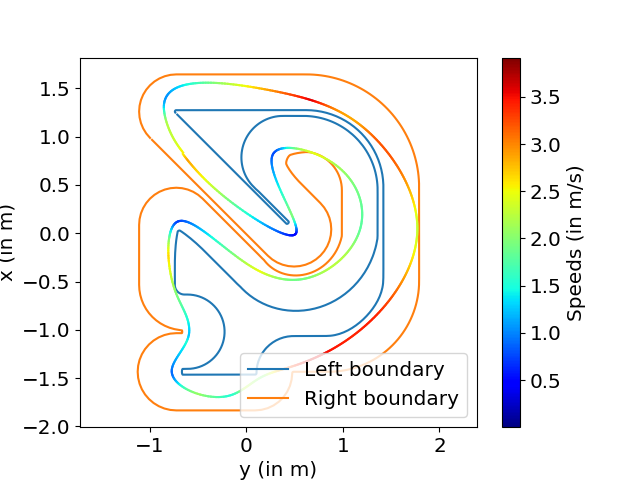
\includegraphics[width=6cm]{Figures/eg_raceline.png}    \end{subfigure}
%     \begin{subfigure}{} 
%         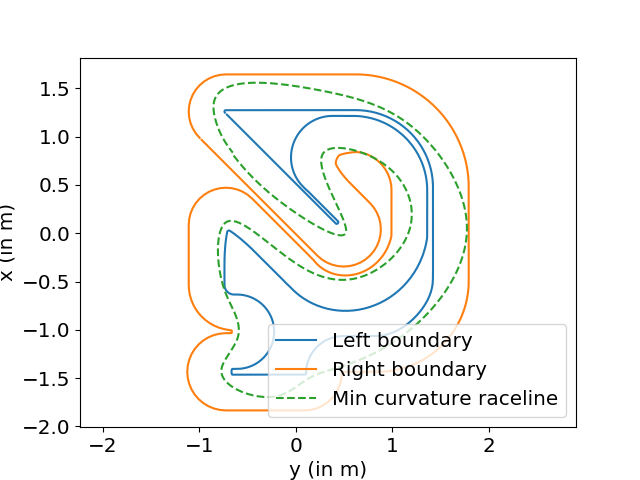
\includegraphics[width=6cm]{Figures/min_curvature_raceline.png}
%     \end{subfigure}
%     \caption{Example (a) raceline and (b) minimum curvature line on a track meant for $1/31^{\text{th}}$ scale racecar}
%     \label{fig:raceline_eg}
% \end{figure}

% \subsection{Formulating it as a Markov game}
% \begin{itemize}
% \item \textbf{Players:} The number of racing cars, denoted by set \(I\). 
%     \item \textbf{State Space:} Location of \((l_i^t,e_i^t)_{i\in I, t\in [N]}\), where \(l_i^t\) denote the longitudinal location of car \(i\) on the racing line at time \(t\) in the future, and \(e_i^t\) is the lateral location of car \(i\) perpendicular to the racing line at time \(t\). 
%     \item \textbf{Action Space:} The action variables at the end of every player is the actions \(u_i\) taken by players (which are determined by solving the raceline tracking problem). 
%     \item \textbf{Policy:}
%     Define a policy to be a mapping \(\pi_i: S\rightarrow A_i\). Note that we only consider deterministic policies. 
%     We parameterize the policies by four tuple \((q,\alpha,\gamma,\lambda)\) where \(q\) is the weight matrix, \(\alpha, \gamma\) are scaling parameters and \(\lambda\) is the safety parameter. 
%     We denote the set of available parameters by the finite set \(\Theta\). 
%     \item \textbf{Transition Function:} The transition function of state is the natural transition function that is based on the current state of the players and resulting trajectory from the optimizatio problem at the end of agents. {\color{red}I think here we are assuming that the players have access to the future \(N\) time step trajectory of other players.}
%     \item \textbf{Utility of players}: The utility of players is determined by the progress along the track. 
%     \begin{align*}
%         u_i(s^k, a^k) = l_i^{k,N} - \max_{j\neq i}l_j^{k,N}
%     \end{align*}
%     \item The initial 
% state is a priori fixed because all players initial state is a fixed location on the racing line 
% \end{itemize}


% The players are non-myopic and wants to maximize the long horizon utility 
% \begin{align*}
%     V_i(s,\pi) = \sum_{k=0}^{T}u_i^k(s^k, a^k)
% \end{align*}
% where \(s^0\) is given and \(a^k = \pi(s^k)\) and \(s^{k+1} = P(\cdot|s^k,a^k)\), and \(T\) is a long horizon time when the race finishes.  




\begin{figure}
    \centering
    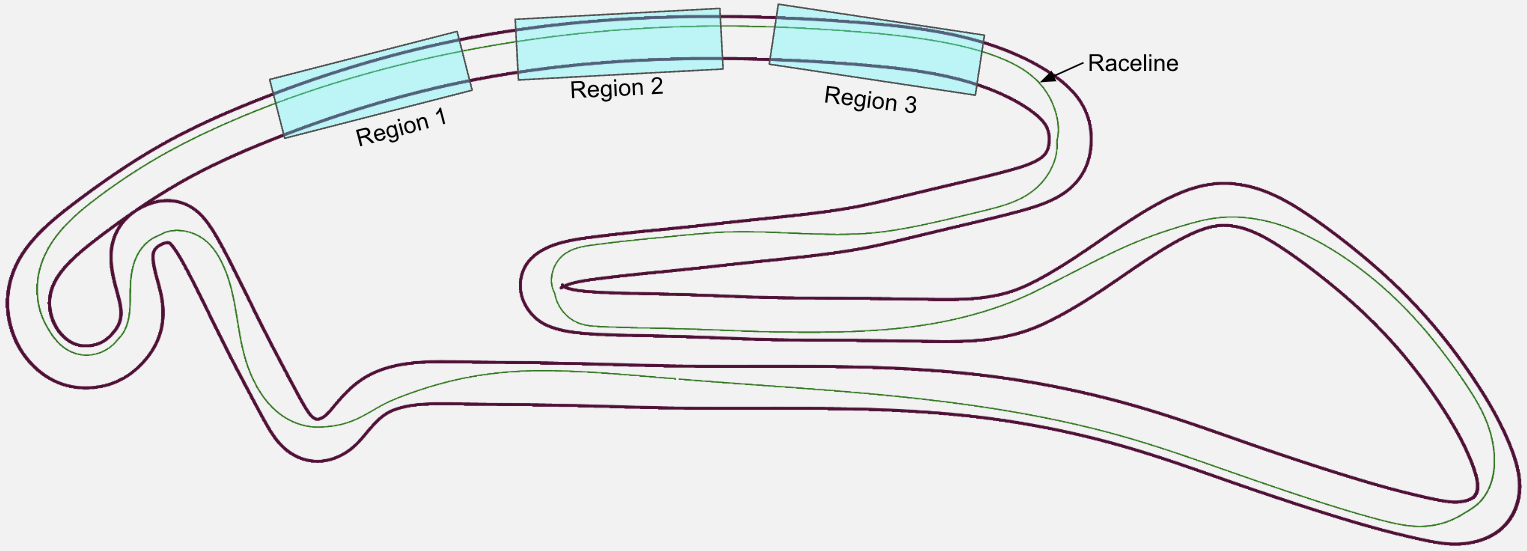
\includegraphics[width=\linewidth]{Figures/racetrack.png}
    \caption{Track and the starting position regions}
    \label{fig:track}
\end{figure}
